\section{Theorie}
\label{sec:Theorie}

\subsection{sec:Austrittsarbeit und Energie}
\label{sec:Austrittsarbeit und Energie}
Werden Metalle erhitzt, treten aus der Oberfläche Elektronen aus.
Diese Elektronenemission wird als \textit{glühelektrischer Effekt} bezeichnet.
Werden Metalle erhitzt, treten aus der
\begin{wrapfigure}{r}{0.4\linewidth}
    \caption{Darstellung eines sogenannten Potentialtopfes}\label{fig:Potentialtopf}
    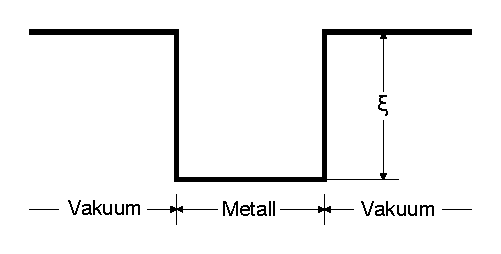
\includegraphics[width=\linewidth]{pictures/Potentialtopf.pdf}
\end{wrapfigure} 
Oberfläche Elektronen aus.
Werden Metalle erhitzt, treten aus der Oberfläche Elektronen aus.
Dafür müssen diese aber zunächst die \textit{Austrittsarbeit} $e_0 \xi$ leisten.
Dabei sit $\xi$ das Potential, welches in \hyperref[fig:Potentialtopf]{Abbildung \ref{fig:Potentialtopf}} anschaulich dargestellt wurde, und
$e_0$ ist die Elementarladung.
Elektronen haben immer eine Energie die von null verschieden ist.
Das wird durch das Pauliprinzip auch am absoluten Temperaturnullpunkt garantiert.
Die Wahrscheinlichkeit , dass im thermischen Gleichgewicht ein Zustand mit einer Energie $E$ besetzt ist, wird durch die
\textit{Fermi-Dirac'sche Verteilungsfunktion}
\begin{equation}
    f(E)=\frac{1}{\exp \left(\frac{E-\zeta}{k T}\right)+1}
\end{equation}
beschrieben. Dabei beschreibt $\zeta$ die \textit{Fermische Grenzenergie}, $k$ die Boltzmann-Konstante und $T$ die Temperatur.

\subsection{Richardson-Gleichung}
\label{eq:Richardson}
Die Sättigungsstromdichte wird durch die sogenannte \textit{Richardson-Gleichung} \cite{v504} beschrieben. Sie lautet
\begin{equation}
    j_{S}(T)=4 \pi \frac{e_{0} m_{0} k^{2}}{h^{3}} T^{2} \exp \left(\frac{-e_{0} \Phi}{k T}\right) .
\end{equation}
\subsection{Hochvakuum-Diode}
Für die Messung des Sättigungsstromes ist eine Hochvakuum-Diode nötig, da sonst die freien Elektronen mit den Gasmolekülen wechselwirken würden.
\begin{figure} [H]
    \center
    \caption{Schematische Darstellung einer Hochvakuum-Diode}\label{fig:Diode}
    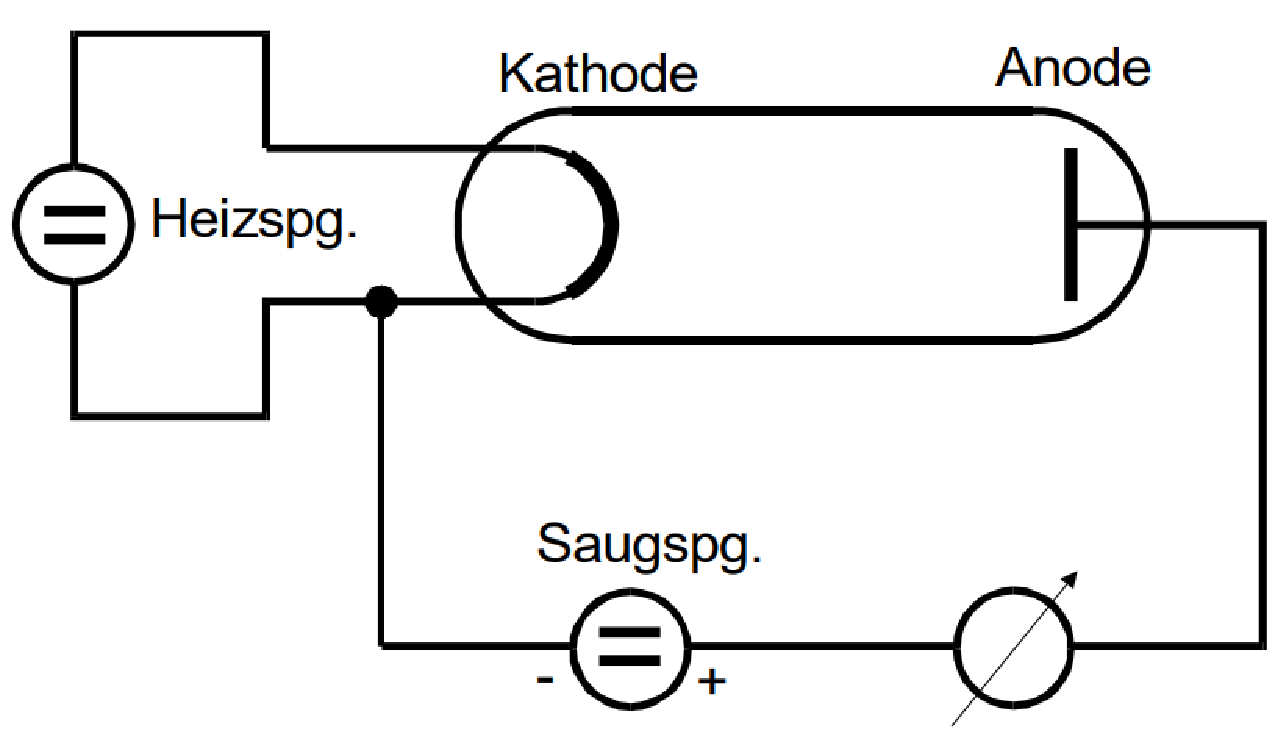
\includegraphics[width=0.5\linewidth]{pictures/Diode.pdf}
\end{figure}
Innerhalb der Diode wird durch die Anode ein elektrisches Feld angelegt, durch welches die Elektronen \enquote{abgesaugt} werden.
Die Elektronen werden durch die Heizspannung an der Kathode abgegeben.